\subsection{Comparación de los sistemas al mismo tamaño}

\begin{figure*}[h!]
    \centering
    \begin{subfigure}{.575\textwidth}
        \centering
        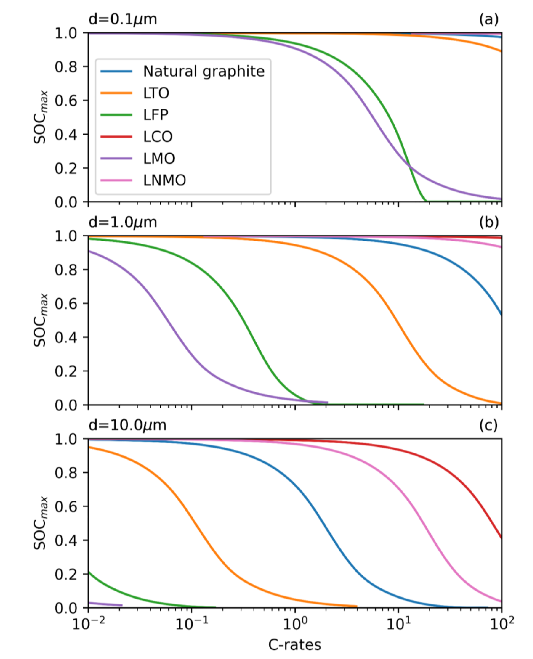
\includegraphics[height=.4\textheight]{FastCharging/un/resultados/comparacion/comparacion-curvas.png}
        \caption{Gráficos SOC$_{\max}$ \textit{versus} C-rate.}
        \label{fig:comparacion-curvas}
    \end{subfigure}
    \begin{subfigure}{.375\textwidth}
        \centering
        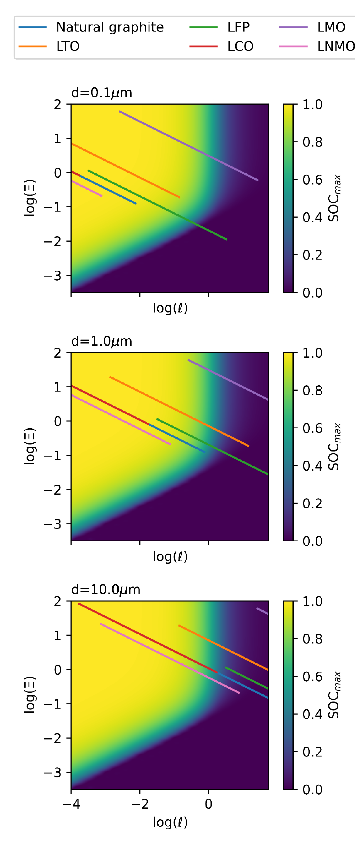
\includegraphics[height=.4\textheight]{FastCharging/un/resultados/comparacion/comparacion-mapa.png}
        \caption{Diagramas.}
        \label{fig:comparacion-mapa}
    \end{subfigure}
    \caption{Comparación de los sistemas considerados con distintos tamaños de 
    partícula entre 0.1 $\mu$m y 10.0 $\mu$m en el rango experimental usual para 
    valores de C-rates.}
    \label{fig:comparacion}
\end{figure*}
